\documentclass[12pt,letterpaper]{report}
\usepackage[margin=1in]{geometry}
\usepackage{titlesec}
\usepackage{amsmath}
\usepackage{amssymb}
\usepackage{subfig}
\usepackage[colorlinks=true,urlcolor=black,linkcolor=black]{hyperref}
\usepackage{graphicx}
\usepackage{textcomp}
\usepackage{mathptmx}
\usepackage{tablefootnote}
\usepackage{array,multirow}
\date{}
\usepackage{multirow}
\usepackage{array}
\usepackage{fullpage}
\usepackage{setspace}
\usepackage{hyperref}

\begin{document}
\begin{figure}
    \centering
    \begin{center}
          
\includegraphics[width=0.8\linewidth]{Images/Concordia_banner.jpg}
    \end{center}
\end{figure}
    \title{SOEN 6431 - Software Comprehension And Maintenance\\[1em]

Deliverable 2 - Reengineering Opportunity\\ \textbf{DÉJÀ VU}}

\newcolumntype{C}[1]{>{\centering\arraybackslash}m{#1}}

\author{Submitted to : Dr. Pankaj Kamthan \\ \\
Summarized by:\\
A K M Saifun Nabi(40222168)\\
Dhruviben Jigeshkumar Modi(40166396)\\
Sumit Vasharambhai Monapara(40197174)\\
Harshal Jigeshkumar Modi (40195060)\\
\\\\
\centering
\href{https://github.com/mdhruvi/SOEN-6431-Deja-Vu}{Github Repository Link}\\
}
\maketitle
\pagebreak

\tableofcontents

\newpage
\addcontentsline{toc}{section}{1. Abstract}
\section*{1. Abstract}
\normalsize {Continuous evolution is essential for a software system's long-term market success. As part of this evolution, the original software must be continuously updated and improved in order to meet the shifting needs of the market. Software maintenance is the term used to describe this ongoing improvement process. It is crucial to carefully examine the source code and documentation and have a deep understanding of the system in order to carry out software maintenance and apply beneficial modifications.\\

We have chosen the R system called Billing System from the 4 candidate systems which we described in deliverable 1. In this deliverable 2, we make changes in source code R as we mentioned in deliverable 1. In this assignment, we make a report about the change in relevant software metrics before and after the re-engineering.
}


\addcontentsline{toc}{section}{2. Introduction}
\section*{2. Introduction}
\normalsize {
Software re-engineering offers numerous advantages such as improved maintainability, enhanced performance, and increased flexibility. Debugging, reviewing, and testing of source code play critical roles in ensuring software reliability, identifying and resolving defects, and enhancing overall code quality. These practices contribute to the development of robust and stable software systems, leading to better user experiences and increased customer satisfaction.\\

The Billing System is a comprehensive store billing application developed in Java with a user-friendly graphical user interface (GUI). The system generates invoices tailored to each state's requirements. The main file, AdminPanel.java, facilitates various CRUD operations such as adding, deleting, and updating products. Additional Java files like updateProduct.java, deleteCashier.java, deleteProduct.java, showStocks.java, and addCashier.java handle specific tasks related to managing products, cashiers, and displaying stock information. Together, these files create an efficient and versatile billing system for stores. \\  

Choosing a Java billing system project based on the team's familiarity with the language provides several benefits, including enhanced collaboration, reduced learning curve, and improved productivity. Implementing the project with the MVC design pattern ensures a proper coding structure, modularity, and maintainability. The effective utilization of Java's exception handling mechanism further enhances the system's reliability and stability. To ensure efficient operations, seamless integration with databases is necessary. This integration facilitates the storage, retrieval, and manipulation of critical data, allowing accurate billing processes, streamlined reporting, and comprehensive analysis. Proper database integration ensures data consistency, security, and scalability. This System has utilized JDBC API. The JDBC API provides a standardized set of interfaces, allowing Java applications to establish connections with various databases. It simplifies database interactions by providing methods to execute SQL queries, retrieve data, and manage transactions.
}

\addcontentsline{toc}{section}{3. List of Source Code Undesirables}
\section*{3. List of Source Code Undesirables}
\normalsize {
Our team has extensively utilized the SonarQube tool to diligently scrutinize our deliverable and detect any undesired elements present in the codebase. The findings we encountered cover a wide spectrum of undesirables, including critical issues such as use of the deprecated libraries, potential security vulnerabilities, and architectural weaknesses, as well as less critical matters such as coding style inconsistencies and suboptimal code blocks.\\

In this section, we present a detailed breakdown of each identified undesirable, providing comprehensive information such as its type, category, specific code smell type, and a comprehensive description. We aim to offer a profound understanding of each issue to facilitate effective resolution and enhance the overall quality of our deliverable.
Throughout this meticulous process, we have meticulously documented a summary for each code smell, providing an overview of its impact on the codebase and potential implications. In total, we have identified and resolved a total of 20 findings, signifying our unwavering commitment to producing a high-quality deliverable that adheres to industry best practices and standards.\\

We have categorized three types of undesirables with their respective explanations: Bugs, Vulnerabilities, and Code Smells.

\textbf{Bug}: A bug refers to an error, flaw, or unintended behavior in the software code that leads to incorrect or unexpected results during execution.

\textbf{Vulnerability}: A vulnerability is a weakness in the software system that could be exploited by an attacker to compromise its security, integrity, or availability.

\textbf{Code Smell}: Code smell indicates a piece of code that is poorly designed or written, making it difficult to maintain, understand, or extend. It doesn't necessarily lead to bugs but hinders code quality and may increase the likelihood of introducing defects.\\
}
\\
\\
\begin{table}[h!]
    \begin{tabular}{|c|c|p{0.7\linewidth}|}
    \hline   
    \multirow{6}{*}{1}
        & Type & Bug \\
    \cline{2-3}
        & Severity & Blocker \\
    \cline{2-3}
       & Observation & Use try-with-resources or close this "Statement" in a "finally" clause. \\
    \cline{2-3}
       & Code Smell Type &  Resource Management - Finally block clean-up\\
    \cline{2-3}
       & Code Smell Summary & Resources like connections, streams, and other classes that implement the Closeable interface should be closedin order to release system resources properly.  \\
    \cline{2-3}
       & Frequency & 16 \\
    \hline
    \end{tabular}
\end{table}


\begin{table} 
    \begin{tabular}{|c|c|p{0.7\linewidth}|}
    \hline   
    \multirow{6}{*}{2}
        & Type & Bug \\
    \cline{2-3}
        & Severity & Major \\
    \cline{2-3}
       & Observation & A "NullPointerException" could be thrown; "conn" is nullable here. \\
    \cline{2-3}
       & Code Smell Type &  Implementation Smells - Null Pointer Dereference.\\
    \cline{2-3}
       & Code Smell Summary & Attempting to dereference or access members/methods of a reference that is null will cause a "NullPointerException," leading to abrupt program termination. We should always perform null checks on nullable references before accessing them. \\
    \cline{2-3}
       & Frequency & 15 \\
    \hline
    \end{tabular}
\end{table}


\begin{table}
    \begin{tabular}{|c|c|p{0.7\linewidth}|}
    \hline   
    \multirow{6}{*}{3}
        & Type & Vulnerability \\
    \cline{2-3}
        & Severity & Blocker \\
    \cline{2-3}
       & Observation & Add password protection to this database. \\
    \cline{2-3}
       & Code Smell Type &  Inadequate Security Measures\\
    \cline{2-3}
       & Code Smell Summary & When relying on the password authentication mode for the database connection, a secure password should be chosen. This rule raises an issue when an empty password is used. \\
    \cline{2-3}
       & Frequency & 1 \\
    \hline
    \end{tabular}
\end{table}

\begin{table}
    \begin{tabular}{|c|c|p{0.7\linewidth}|}
    \hline   
    \multirow{6}{*}{4}
        & Type & Code Smell \\
    \cline{2-3}
        & Severity & Critical \\
    \cline{2-3}
       & Observation & Use static access with \textbf{javax.swing.WindowConstants} for DISPOSE\_ON\_CLOSE \\
    \cline{2-3}
       & Code Smell Type &  Static Overuse: Excessive Static Access. \\
    \cline{2-3}
       & Code Smell Summary & In the interest of code clarity, static members of a base class should never be accessed using a derived type’s name. Doing so is confusing and could create the illusion that two different static members exist. \\
    \cline{2-3}
       & Frequency & 2 \\
    \hline
    \end{tabular}
\end{table}

\begin{table}
    \begin{tabular}{|c|c|p{0.7\linewidth}|}
    \hline   
    \multirow{6}{*}{5}
        & Type & Code Smell \\
    \cline{2-3}
        & Severity & Critical \\
    \cline{2-3}
       & Observation & Define a constant instead of duplicating this literal \textbf{"XXXX"} N times. \\
    \cline{2-3}
       & Code Smell Type &  Duplicated Variable - Magic String \\
    \cline{2-3}
       & Code Smell Summary & Duplicated string literals make the process of refactoring error-prone since you must be sure to update all occurrences, but with assigning to constant, we need to update only once and access anywhere. \\
    \cline{2-3}
       & Frequency & 25 \\
    \hline
    \end{tabular}
\end{table}


\begin{table}
    \begin{tabular}{|c|c|p{0.7\linewidth}|}
    \hline   
    \multirow{6}{*}{6}
        & Type & Code Smell \\
    \cline{2-3}
        & Severity & Critical \\
    \cline{2-3}
       & Observation & Add a nested comment explaining why this method is empty or throw Exception \\
    \cline{2-3}
       & Code Smell Type & Configuration Smells : Empty method  \\
    \cline{2-3}
       & Code Smell Summary & There are several reasons for a method not to have a method body: if the method will not be used in the future, throw an UnSupportedOperationException or if overriding it, add a nested comment explaining why this method is empty. \\
    \cline{2-3}
       & Frequency & 1 \\
    \hline
    \end{tabular}
\end{table}

\begin{table}
    \begin{tabular}{|c|c|p{0.7\linewidth}|}
    \hline   
    \multirow{6}{*}{7}
        & Type & Code Smell \\
    \cline{2-3}
        & Severity & Critical \\
    \cline{2-3}
       & Observation & Make \textbf{"XXXX"} transient or serializable. \\
    \cline{2-3}
       & Code Smell Type & Implementation Smells: Serialization Smell  \\
    \cline{2-3}
       & Code Smell Summary & Fields in a Serializable class must themselves be either Serializable or transient,even if the class is never explicitly serialized or deserialized. This rule raises an issue on non-Serializable fields. \\
    \cline{2-3}
       & Frequency & 1 \\
    \hline
    \end{tabular}
\end{table}

\begin{table}
    \begin{tabular}{|c|c|p{0.7\linewidth}|}
    \hline   
    \multirow{6}{*}{8}
        & Type & Code Smell \\
    \cline{2-3}
        & Severity & Critical \\
    \cline{2-3}
       & Observation & Refactor this method to reduce its Cognitive Complexity from 23 to the 15 allowed. \\
    \cline{2-3}
       & Code Smell Type & Complex code: High Cognitive Complexity  \\
    \cline{2-3}
       & Code Smell Summary & Cognitive Complexity is a measure of how hard the control flow of a method is to understand. Methods with high Cognitive Complexity will be difficult to maintain. \\
    \cline{2-3}
       & Frequency & 2 \\
    \hline
    \end{tabular}
\end{table}

\begin{table}
    \begin{tabular}{|c|c|p{0.7\linewidth}|}
    \hline   
    \multirow{6}{*}{9}
        & Type & Code Smell \\
    \cline{2-3}
        & Severity & Critical \\
    \cline{2-3}
       & Observation & Use static access with \textbf{javax.swing.WindowConstants} for "EXIT\_ON\_CLOSE" \\
    \cline{2-3}
       & Code Smell Type & Static Overuse: Excessive Static Access  \\
    \cline{2-3}
       & Code Smell Summary & In the interest of code clarity, static members of a base class should never be accessed using a derived type’s name. Doing so is confusing and could create the illusion that two different static members exist. \\
    \cline{2-3}
       & Frequency & 1 \\
    \hline
    \end{tabular}
\end{table}

\begin{table}
    \begin{tabular}{|c|c|p{0.7\linewidth}|}
    \hline   
    \multirow{6}{*}{10}
        & Type & Code Smell \\
    \cline{2-3}
        & Severity & Critical \\
    \cline{2-3}
       & Observation & Add a default case to this switch. \\
    \cline{2-3}
       & Code Smell Type & Switch statements   \\
    \cline{2-3}
       & Code Smell Summary & The requirement for a final default clause is defensive programming. The clause should either take appropriate action, or contain a suitable comment as to why no action is taken. \\
    \cline{2-3}
       & Frequency & 3 \\
    \hline
    \end{tabular}
\end{table}

\begin{table}
    \begin{tabular}{|c|c|p{0.7\linewidth}|}
    \hline   
    \multirow{6}{*}{11}
        & Type & Code Smell \\
    \cline{2-3}
        & Severity & Major \\
    \cline{2-3}
       & Observation & Replace this use of \textbf{System.out \textbackslash System.err} by a \textbf{logger}. \\
    \cline{2-3}
       & Code Smell Type & Implementation Smells: Logging   \\
    \cline{2-3}
       & Code Smell Summary & Everyone must follow the logging patterns to easily retrieve the logs for all users, the format of the log should be uniform across applications, and logged data must be recorded for future use. \\
    \cline{2-3}
       & Frequency & 3 \\
    \hline
    \end{tabular}
\end{table}

\begin{table}
    \begin{tabular}{|c|c|p{0.7\linewidth}|}
    \hline   
    \multirow{6}{*}{12}
        & Type & Code Smell \\
    \cline{2-3}
        & Severity & Major \\
    \cline{2-3}
       & Observation & Make this anonymous inner class a lambda. \\
    \cline{2-3}
       & Code Smell Type & Anonymous Class Smell   \\
    \cline{2-3}
       & Code Smell Summary & Before Java 8, the only way to partially support closures in Java was by using anonymous inner classes, but the syntax was unclear and unwieldy, so after Java 8, anonymous inner classes should be replaced by lambdas to highly increase the readability. \\
    \cline{2-3}
       & Frequency & 22 \\
    \hline
    \end{tabular}
\end{table}

\begin{table}
    \begin{tabular}{|c|c|p{0.7\linewidth}|}
    \hline   
    \multirow{6}{*}{13}
        & Type & Code Smell \\
    \cline{2-3}
        & Severity & Major \\
    \cline{2-3}
       & Observation & This block of commented-out lines of code should be removed. \\
    \cline{2-3}
       & Code Smell Type & Implementation Smells - Comments   \\
    \cline{2-3}
       & Code Smell Summary & Programmers should not comment out code as it bloats programs and reduces readability. Unused code should be deleted and can be retrieved from source control history if required \\
    \cline{2-3}
       & Frequency & 7 \\
    \hline
    \end{tabular}
\end{table}

\begin{table}
    \begin{tabular}{|c|c|p{0.7\linewidth}|}
    \hline   
    \multirow{6}{*}{14}
        & Type & Code Smell \\
    \cline{2-3}
        & Severity & Major \\
    \cline{2-3}
       & Observation & Remove this useless assignment to local variable \textbf{"XXXX"}. \\
    \cline{2-3}
       & Code Smell Type & Resource Management - Dead Store   \\
    \cline{2-3}
       & Code Smell Summary &  dead store happens when a local variable is assigned a value that is not read by any subsequent instruction and leads to waste of storage, Therefore all calculated values should be used. \\
    \cline{2-3}
       & Frequency & 4 \\
    \hline
    \end{tabular}
\end{table}

\begin{table}
    \begin{tabular}{|c|c|p{0.7\linewidth}|}
    \hline   
    \multirow{6}{*}{15}
        & Type & Code Smell \\
    \cline{2-3}
        & Severity & Minor \\
    \cline{2-3}
       & Observation & Rename this class name to match the regular expression '\^[A-Z][a-zA-Z0-9]*\$'.. \\
    \cline{2-3}
       & Code Smell Type & Configuration Smells : Inconsistent Naming Convention  \\
    \cline{2-3}
       & Code Smell Summary &  Shared coding conventions allow teams to collaborate effectively. This rule allows us to check that all class names match a provided regular expression.. \\
    \cline{2-3}
       & Frequency & 9 \\
    \hline
    \end{tabular}
\end{table}

\begin{table}
    \begin{tabular}{|c|c|p{0.7\linewidth}|}
    \hline   
    \multirow{6}{*}{16}
        & Type & Code Smell \\
    \cline{2-3}
        & Severity & Minor \\
    \cline{2-3}
       & Observation & Remove this unused import \textbf{"AB.CD.EF"}. \\
    \cline{2-3}
       & Code Smell Type & Architectural Smells - Unused Packages   \\
    \cline{2-3}
       & Code Smell Summary &  The import part of a file should be handled by the Integrated Development Environment (IDE), not manually by the developer. Leaving them in reduces the code’s readability since their presence can be confusing. \\
    \cline{2-3}
       & Frequency & 28 \\
    \hline
    \end{tabular}
\end{table}

\begin{table}
    \begin{tabular}{|c|c|p{0.7\linewidth}|}
    \hline   
    \multirow{6}{*}{17}
        & Type & Code Smell \\
    \cline{2-3}
        & Severity & Info \\
    \cline{2-3}
       & Observation & Complete the task associated to this TODO comment.. \\
    \cline{2-3}
       & Code Smell Type & Implementation Smells :  Comments   \\
    \cline{2-3}
       & Code Smell Summary &  \textbf{TODO} tags are commonly used to mark places where some more code is required, but which the developer wants to implement later. This rule is meant to track those tags and to ensure that they do not go unnoticed. \\
    \cline{2-3}
       & Frequency & 26 \\
    \hline
    \end{tabular}
\end{table}

\begin{figure}
    \centering
    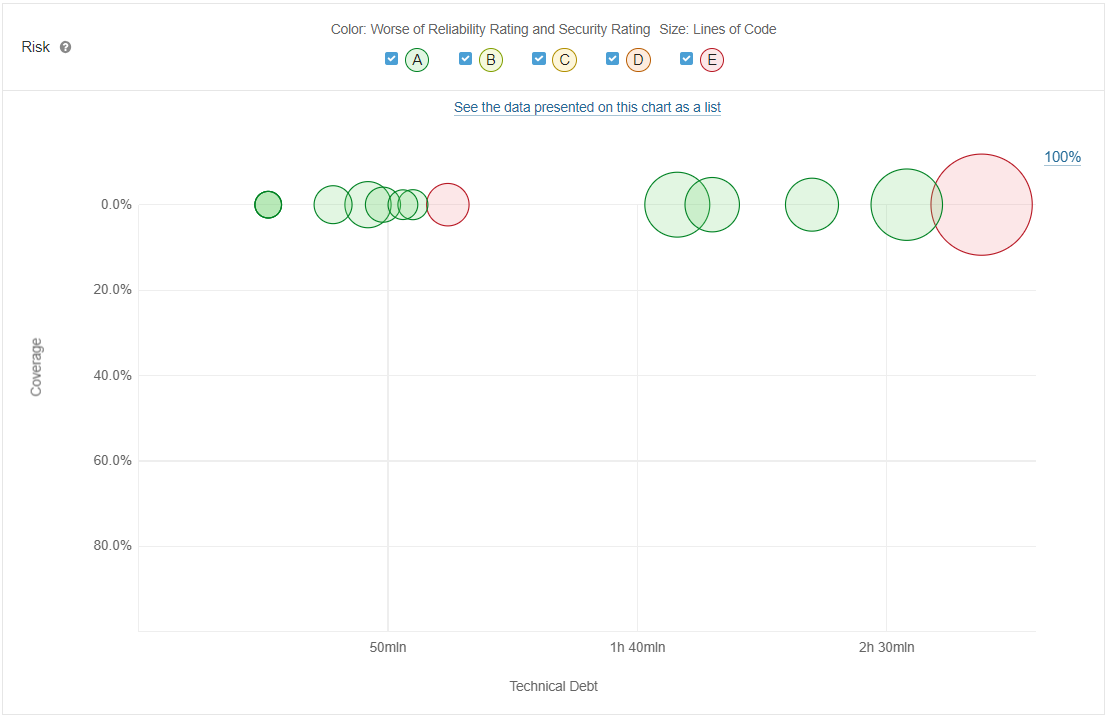
\includegraphics[width=0.7\linewidth]{Images/Debt_per_class.png}\
    \caption{SonarQube Analysis of issues per Java class (Billing System)}
    \label{fig:enter-label}
\end{figure}

\begin{figure}
    \centering
    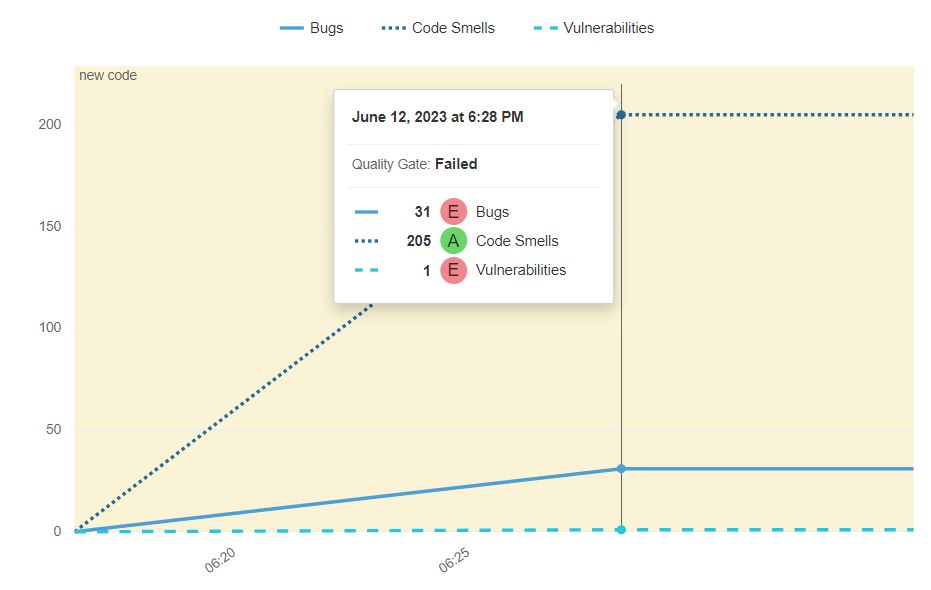
\includegraphics[width=0.7\linewidth]{Images/Issue_commit.jpg}\
    \caption{SonarQube Analysis of Each undesirables (Billing System)}
    \label{fig:enter-label}
\end{figure}
\pagebreak

\addcontentsline{toc}{section}{4. Re-engineering Methods for Undesrirables} 
\section*{4. Re-engineering Methods for Undesrirables}
\normalsize {
In this particular section, we have provided a comprehensive account of the mapping process between source code undesirables and the corresponding re-engineering methods. Our aim was to establish a clear association between the observed undesirables and the appropriate re-engineering rule, rule type, issue tag, undesirable severity, undesirable likelihood, technical debt.\\

Since our chosen system is implemented in Java, we employed Java Static Code Analysis as a valuable tool for this endeavor. Relying on the insights gained from this analysis, we were able to accurately identify and categorize the aforementioned elements, ensuring a systematic and methodical approach to the evaluation.\\

By leveraging the insights derived from the Java Static Code Analysis graph, we could confidently pinpoint and assess the significance of each mapping, ultimately leading us to make informed decisions on how best to address the identified undesirables and implement the suitable reengineering methods. This approach fosters a well-organized and targeted strategy for optimizing the system's code quality and overall performance.\\

\begin{figure}[h!]
    \centering
    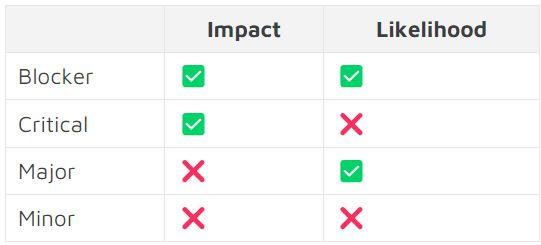
\includegraphics[width=0.7\linewidth]{Images/Severity_report.jpeg}\
    \caption{SonarQube Analysis of Severity Category}
    \label{fig:enter-label}
\end{figure}

\begin{table}
    \begin{tabular}{|c|c|p{0.7\linewidth}|}
    \hline   
    \multirow{8}{*}{1}
        & Re-engineering Rule Type & Bug \\
    \cline{2-3}
       & Severity &  Blocker \\
    \cline{2-3}
       & Likelihood &  High \\
    \cline{2-3}
       & Observation & Use try-with-resources or close this "Statement" in a "finally" clause. \\
    \cline{2-3}
        & Re-engineering Rule Description & Connections, streams, files, and other classes that implement the Closeable interface or its super-interface, AutoCloseable, needs to be closed after use. Further, that close call must be made in a finally block otherwise an exception could keep the call from being made. Preferably, when a class implements AutoCloseable, the "try-with-resources" pattern should be used to ensure automatic resource cleanup \\
    \cline{2-3}
       & Issue Tag & \href{https://cwe.mitre.org/data/definitions/459}{cwe-459}, bad practice, \href{https://wiki.sei.cmu.edu/confluence/display/java/FIO04-J.+Release+resources+when+they+are+no+longer+needed}{cert - FIO04-J}  \\
    \cline{2-3}
       & Technical Debt & 80 min effort  \\
    \cline{2-3}
       & Refactored By & Sumit Monapara \\
    \hline
    \end{tabular}
\end{table}

\begin{table}
    \begin{tabular}{|c|c|p{0.7\linewidth}|}
    \hline   
    \multirow{8}{*}{2}
        & Re-engineering Rule Type & Bug \\
    \cline{2-3}
       & Severity &  Major \\
    \cline{2-3}
       & Likelihood &  High \\
    \cline{2-3}
       & Observation & A "NullPointerException" could be thrown; "conn" is nullable here. \\
    \cline{2-3}
       & Re-engineering Rule Description & A reference to null should never be dereferenced/accessed. Doing so will cause a NullPointerException to be thrown. At best, such an exception will cause abrupt program termination. At worst, it could expose debugging information that would be useful to an attacker, or it could allow an attacker to bypass security measures.  \\
    \cline{2-3}
       & Issue Tag & \href{https://cwe.mitre.org/data/definitions/476}{cwe-476}, \href{https://wiki.sei.cmu.edu/confluence/display/java/EXP01-J.+Do+not+use+a+null+in+a+case+where+an+object+is+required}{cert - EXP01-J}, bad practice  \\
    \cline{2-3}
       & Technical Debt & 120 min effort  \\
    \cline{2-3}
       & Refactored By & Sumit Monapara \\
    \hline
    \end{tabular}
\end{table}

\begin{table}
    \begin{tabular}{|c|c|p{0.7\linewidth}|}
    \hline   
    \multirow{8}{*}{3}
        & Re-engineering Rule Type & Vulnerability \\
    \cline{2-3}
       & Severity &  Blocker \\
    \cline{2-3}
       & Likelihood &  Rare \\
    \cline{2-3}
       & Observation & Add password protection to this database. \\
    \cline{2-3}
       & Re-engineering Rule Description & When utilizing password authentication for the database connection, it is crucial to select a secure password. An issue arises when an empty password is employed.  \\
    \cline{2-3}
       & Issue Tag & \href{https://cwe.mitre.org/data/definitions/521}{cwe-521}, \href{https://owasp.org/www-project-top-ten/2017/A3_2017-Sensitive_Data_Exposure}{OWASP-A3} \\
    \cline{2-3}
       & Technical Debt & 45 min effort  \\
    \cline{2-3}
       & Refactored By & Sumit Monapara \\
    \hline
    \end{tabular}
\end{table}

\begin{table}
    \begin{tabular}{|c|c|p{0.7\linewidth}|}
    \hline   
    \multirow{8}{*}{4}
        & Re-engineering Rule Type & Code Smell \\
    \cline{2-3}
       & Severity &  Critical \\
    \cline{2-3}
       & Likelihood &  Rare \\
    \cline{2-3}
       & Observation & Use static access with \textbf{javax.swing.WindowConstants} for DISPOSE\_ON\_CLOSE \\
    \cline{2-3}
       & Re-engineering Rule Description & To maintain code clarity, avoid accessing static members of a base class using the name of a derived type. This practice can lead to confusion and may wrongly imply the existence of two distinct static members.  \\
    \cline{2-3}
       & Issue Tag & confusing \\
    \cline{2-3}
       & Technical Debt & 5 min effort  \\
    \cline{2-3}
       & Refactored By & Harshal Modi \\
    \hline
    \end{tabular}
\end{table}

\begin{table}
    \begin{tabular}{|c|c|p{0.7\linewidth}|}
    \hline   
    \multirow{8}{*}{5}
        & Re-engineering Rule Type & Code Smell \\
    \cline{2-3}
       & Severity &  Critical \\
    \cline{2-3}
       & Likelihood &  Rare \\
    \cline{2-3}
       & Observation & Define a constant instead of duplicating this literal \textbf{"XXXX"} N times. \\
    \cline{2-3}
       & Re-engineering Rule Description & By duplicating Literals, we must be sure to update all occurrences. On the other hand, constants can be referenced from many places, but only need to be updated in a single place.  \\
    \cline{2-3}
       & Issue Tag & design, duplicate \\
    \cline{2-3}
       & Technical Debt & 225 min effort  \\
    \cline{2-3}
       & Refactored By & Sumit Monapara \\
    \hline
    \end{tabular}
\end{table}

\begin{table}
    \begin{tabular}{|c|c|p{0.7\linewidth}|}
    \hline   
    \multirow{8}{*}{6}
        & Re-engineering Rule Type & Code Smell \\
    \cline{2-3}
       & Severity &  Critical \\
    \cline{2-3}
       & Likelihood &  Rare \\
    \cline{2-3}
       & Observation & Add a nested comment explaining why this method is empty or throw Exception. \\
    \cline{2-3}
       & Re-engineering Rule Description &  There are many reasons to have a method without a body: if the method will not be used in the future, throw an UnSupportedOperationException or if overriding it, add a nested comment explaining why this method is empty. \\
    \cline{2-3}
       & Issue Tag & suspicious \\
    \cline{2-3}
       & Technical Debt & 5 min effort  \\
    \cline{2-3}
       & Refactored By & Harshal Modi \\
    \hline
    \end{tabular}
\end{table}

\begin{table}
    \begin{tabular}{|c|c|p{0.7\linewidth}|}
    \hline   
    \multirow{8}{*}{7}
        & Re-engineering Rule Type & Code Smell \\
    \cline{2-3}
       & Severity &  Critical \\
    \cline{2-3}
       & Likelihood &  Rare \\
    \cline{2-3}
       & Observation & \textbf{"XXXX"} transient or serializable. \\
    \cline{2-3}
       & Re-engineering Rule Description &  In a Serializable class, all fields must either be Serializable or marked as transient, even if the class is never explicitly serialized or deserialized. This rule highlights potential issues with non-Serializable fields and with collection fields that are not private and are assigned non-Serializable types within the class. \\
    \cline{2-3}
       & Issue Tag & \href{https://cwe.mitre.org/data/definitions/594}{cwe-594}, \href{https://docs.oracle.com/javase/7/docs/api/java/io/Serializable.html}{serialization} \\
    \cline{2-3}
       & Technical Debt & 30 min effort  \\
    \cline{2-3}
       & Refactored By & Harshal Modi \\
    \hline
    \end{tabular}
\end{table}

\begin{table}
    \begin{tabular}{|c|c|p{0.7\linewidth}|}
    \hline   
    \multirow{8}{*}{8}
        & Re-engineering Rule Type & Code Smell \\
    \cline{2-3}
       & Severity &  Critical \\
    \cline{2-3}
       & Likelihood &  Rare \\
    \cline{2-3}
       & Observation & Refactor this method to reduce its Cognitive Complexity from 23 to the 15 allowed. \\
    \cline{2-3}
       & Re-engineering Rule Description & Cognitive Complexity is a measurement of the difficulty in understanding the control flow of a method. Methods with high Cognitive Complexity will be challenging to maintain due to their intricate control structures, making them hard to comprehend and modify.  \\
    \cline{2-3}
       & Issue Tag & brain-overload \\
    \cline{2-3}
       & Technical Debt & 21 min effort  \\
    \cline{2-3}
       & Refactored By & Harshal Modi \\
    \hline
    \end{tabular}
\end{table}

\begin{table}
    \begin{tabular}{|c|c|p{0.7\linewidth}|}
    \hline   
    \multirow{8}{*}{9}
        & Re-engineering Rule Type & Code Smell \\
    \cline{2-3}
       & Severity &  Critical \\
    \cline{2-3}
       & Likelihood &  Rare \\
    \cline{2-3}
       & Observation & Use static access with \textbf{javax.swing.WindowConstants} for "EXIT\_ON\_CLOSE" \\
    \cline{2-3}
       & Re-engineering Rule Description & To maintain code clarity, avoid accessing static members of a base class using the name of a derived type. This practice can lead to confusion and may wrongly imply the existence of two distinct static members.  \\
    \cline{2-3}
       & Issue Tag & confusing \\
    \cline{2-3}
       & Technical Debt & 5 min effort  \\
    \cline{2-3}
       & Refactored By & Harshal Modi \\
    \hline
    \end{tabular}
\end{table}

\begin{table}
    \begin{tabular}{|c|c|p{0.7\linewidth}|}
    \hline   
    \multirow{8}{*}{10}
        & Re-engineering Rule Type & Code Smell \\
    \cline{2-3}
       & Severity &  Critical \\
    \cline{2-3}
       & Likelihood &  High \\
    \cline{2-3}
       & Observation & Add a default case to this switch. \\
    \cline{2-3}
       & Re-engineering Rule Description &  If the switch parameter is an Enum and if all the constants of this enum are used in the case statements, then no default clause is expected. In other cases, we must need a default case to catch the additional conditions that are not caught in other catch blocks. \\
    \cline{2-3}
       & Issue Tag & \href{https://cwe.mitre.org/data/definitions/478}{cwe-478}, \href{https://wiki.sei.cmu.edu/confluence/display/c/MSC01-C.+Strive+for+logical+completeness}{cert-MSC01-C} \\
    \cline{2-3}
       & Technical Debt & 15 min effort  \\
    \cline{2-3}
       & Refactored By & Dhruvi Modi \\
    \hline
    \end{tabular}
\end{table}

\begin{table}
    \begin{tabular}{|c|c|p{0.7\linewidth}|}
    \hline   
    \multirow{8}{*}{11}
        & Re-engineering Rule Type & Code Smell \\
    \cline{2-3}
       & Severity &  Major \\
    \cline{2-3}
       & Likelihood &  Rare \\
    \cline{2-3}
       & Observation & Replace this use of \textbf{System.out \textbackslash System.err} by a \textbf{logger}. \\
    \cline{2-3}
       & Re-engineering Rule Description & Logging messages must meet the below requirements: Users should have convenient access to retrieve the logs. All logged messages must have a consistent format for easy readability.
The logged data must be reliably recorded. Sensitive data should only be logged in a secure manner. To fulfill these requirements, it is highly recommended to define and use a dedicated logger instead of directly writing to standard outputs in a program.  \\
    \cline{2-3}
       & Issue Tag & \href{https://owasp.org/Top10/A09_2021-Security_Logging_and_Monitoring_Failures/}{OWASP-A9}, bad practice, \href{https://wiki.sei.cmu.edu/confluence/display/java/ERR02-J.+Prevent+exceptions+while+logging+data}{cert-ERR02-J} \\
    \cline{2-3}
       & Technical Debt & 30 min effort  \\
    \cline{2-3}
       & Refactored By & Dhruvi Modi \\
    \hline
    \end{tabular}
\end{table}

\begin{table}
    \begin{tabular}{|c|c|p{0.7\linewidth}|}
    \hline   
    \multirow{8}{*}{12}
        & Re-engineering Rule Type & Code Smell \\
    \cline{2-3}
       & Severity &  Major \\
    \cline{2-3}
       & Likelihood &  High \\
    \cline{2-3}
       & Observation & Make this anonymous inner class a lambda. \\
    \cline{2-3}
       & Re-engineering Rule Description & Prior to Java 8, the only method to achieve partial support for closures in Java was through anonymous inner classes. However, the syntax of anonymous classes could be cumbersome and unclear. With the introduction of Java 8, the use of lambdas significantly improved the readability of the source code.  \\
    \cline{2-3}
       & Issue Tag & version greater than java8\\
    \cline{2-3}
       & Technical Debt & 110 min effort  \\
    \cline{2-3}
       & Refactored By & Dhruvi Modi \\
    \hline
    \end{tabular}
\end{table}

\begin{table}
    \begin{tabular}{|c|c|p{0.7\linewidth}|}
    \hline   
    \multirow{8}{*}{13}
        & Re-engineering Rule Type & Code Smell \\
    \cline{2-3}
       & Severity &  Major \\
    \cline{2-3}
       & Likelihood &  Rare\\
    \cline{2-3}
       & Observation & This block of commented-out lines of code should be removed. \\
    \cline{2-3}
       & Re-engineering Rule Description &  Unused code should be deleted and can be retrieved from source control history if required. \\
    \cline{2-3}
       & Issue Tag & unused\\
    \cline{2-3}
       & Technical Debt & 35 min effort  \\
    \cline{2-3}
       & Refactored By & Dhruvi Modi \\
    \hline
    \end{tabular}
\end{table}

\begin{table}
    \begin{tabular}{|c|c|p{0.7\linewidth}|}
    \hline   
    \multirow{8}{*}{14}
        & Re-engineering Rule Type & Code Smell \\
    \cline{2-3}
       & Severity &  Major \\
    \cline{2-3}
       & Likelihood &  Rare\\
    \cline{2-3}
       & Observation & Remove this useless assignment to local variable \textbf{"XXXX"}. \\
    \cline{2-3}
       & Re-engineering Rule Description &  A dead store occurs when a local variable is assigned a value that is not utilized by any subsequent instruction. This situation, where a value is calculated or retrieved but then immediately overwritten or discarded, may indicate a significant coding error. As a result, it is crucial to utilize all calculated values to avoid dead stores in the code. \\
    \cline{2-3}
       & Issue Tag & \href{https://cwe.mitre.org/data/definitions/563}{cwe-563}, \href{https://wiki.sei.cmu.edu/confluence/display/c/MSC13-C.+Detect+and+remove+unused+values}{cert-MSC13-C}, unused\\
    \cline{2-3}
       & Technical Debt & 60 min effort  \\
    \cline{2-3}
       & Refactored By & A K M Saifun Nabi \\
    \hline
    \end{tabular}
\end{table}

\begin{table}
    \begin{tabular}{|c|c|p{0.7\linewidth}|}
    \hline   
    \multirow{8}{*}{15}
        & Re-engineering Rule Type & Code Smell \\
    \cline{2-3}
       & Severity &  Minor \\
    \cline{2-3}
       & Likelihood &  Rare\\
    \cline{2-3}
       & Observation & Rename this class name to match the regular expression '\^[A-Z][a-zA-Z0-9]*\$'.. \\
    \cline{2-3}
       & Re-engineering Rule Description &  Shared naming conventions allow teams to collaborate efficiently. This rule checks that all method names match a provided regular expression. \\
    \cline{2-3}
       & Issue Tag & convention \\
    \cline{2-3}
       & Technical Debt & 45 min effort  \\
    \cline{2-3}
       & Refactored By & A K M Saifun Nabi \\
    \hline
    \end{tabular}
\end{table}

\begin{table}
    \begin{tabular}{|c|c|p{0.7\linewidth}|}
    \hline   
    \multirow{8}{*}{16}
        & Re-engineering Rule Type & Code Smell \\
    \cline{2-3}
       & Severity &  Minor \\
    \cline{2-3}
       & Likelihood &  Rare\\
    \cline{2-3}
       & Observation & Remove this unused import \textbf{"AB.CD.EF"}. \\
    \cline{2-3}
       & Re-engineering Rule Description &  The import part of a file should be handled by the Integrated Development Environment (IDE), not manually by the developer. Unused and useless imports should not occur if that is the case. Leaving them in reduces the code’s readability since their presence can be confusing. \\
    \cline{2-3}
       & Issue Tag & unused \\
    \cline{2-3}
       & Technical Debt & 56 min effort  \\
    \cline{2-3}
       & Refactored By & A K M Saifun Nabi \\
    \hline
    \end{tabular}
\end{table}

\vspace*{0.1 cm}
\begin{table}
    \begin{tabular}{|c|c|p{0.7\linewidth}|}
    \hline   
    \multirow{8}{*}{17}
        & Re-engineering Rule Type & Code Smell \\
    \cline{2-3}
       & Severity &  Info \\
    \cline{2-3}
       & Likelihood &  Rare\\
    \cline{2-3}
       & Observation & Complete the task associated to this TODO comment..  \\
    \cline{2-3}
       & Re-engineering Rule Description &  TODO tags are frequently utilized to indicate areas in the code that require additional implementation but are intended to be addressed later by the developer. However, there is a risk that the developer might forget or not have the time to revisit those tags. This rule is designed to monitor and ensure that these TODO tags are not overlooked or left unaddressed. \\
    \cline{2-3}
       & Issue Tag & \href{https://cwe.mitre.org/data/definitions/546}{cwe-546} \\
    \cline{2-3}
       & Technical Debt & 26 min effort  \\
    \cline{2-3}
       & Refactored By & A K M Saifun Nabi \\
    \hline
    \end{tabular}
\end{table}
\pagebreak
}

\addcontentsline{toc}{section}{5. Occurrences of Source Code Undesirables}
\section*{5. Occurrences of Source Code Undesirables}
\normalsize{
This tabulated data presents a comprehensive summary of the identified undesirables, outlining their specific occurrences within the codebase.  Furthermore, the number of occurrences of different undesirables per file is included, providing a detailed overview of the distribution and prevalence of these undesirables throughout the codebase.\\

\begin{table}[h!]
\begin{tabular}{|l|l|l|l|l|l|l|} 
\hline
\textbf{No.} & \textbf{File} & \textbf{Lines}${}^\star$${}^\star$ & \textbf{Lines of code}${}^\star$ & \textbf{Bug} & \textbf{Vulnerability} & \textbf{Code Smell} \\
\hline
1 & src\textbackslash{addCashier.java} & 81 & 66 & 0 & 0 & 11 \\
\hline
2 & src\textbackslash{addProduct.java} & 112 & 94 & 0 & 0 & 8 \\
\hline
3 & src\textbackslash{AdminPanel.java} & 220 & 189 & 0 & 0 & 15 \\
\hline
4 & src\textbackslash{DB.java} & 359 & 317 & 30 & 1 & 36 \\
\hline
5 & src\textbackslash{deleteCashier.java} & 80 & 65 & 0 & 0 & 10 \\
\hline
6 & src\textbackslash{deleteProduct.java} & 69 & 54 & 0 & 0 & 6 \\
\hline
7 & src\textbackslash{generateInvoice.java} & 109 & 84 & 0 & 0 & 9 \\
\hline
8 & src\textbackslash{Invoice.java} & 250 & 212 & 0 & 0 & 21 \\
\hline
9 & src\textbackslash{Login.java} & 198 & 152 & 0 & 0 & 25\\
\hline
10 & src\textbackslash{Sale.java} & 179 & 147 & 0 & 0 & 24 \\
\hline
11 & src\textbackslash{searchCashier.java} & 69 & 54 & 0 & 0 & 6 \\
\hline
12 & src\textbackslash{searchProduct.java} & 69 & 54 & 0 & 0 & 6 \\
\hline
13 & src\textbackslash{showStock.java} & 132 & 110 & 1 & 0 & 15 \\
\hline
14 & src\textbackslash{updateProduct.java} & 149 & 123 & 0 & 0 & 13 \\
\hline
\hline

 &  & \textbf{LOC : 2076} &\textbf{SLOC : 1721} & \textbf{31} &\textbf{1} & \textbf{205}\\
\hline
\multicolumn{6}{c}{\footnotesize ${}^\star$${}^\star$\textbf{Lines:} Physical lines in the file. \hspace{1cm}  ${}^\star$\textbf{Lines of code:} Actual logical code}
\end{tabular}
\end{table}

Upon examining the table presented above, it becomes evident that the entire codebase consists of \textbf{2076 Lines of Code (LOC) with 1721 Source Lines of Code (SLOC)}. Within this substantial codebase, \textbf{a total of 237 undesirables} were identified, encompassing diverse issues such as bugs, vulnerabilities, and code smells. This comprehensive evaluation provides valuable insights into the overall quality and potential areas of improvement within the software, highlighting the significance of addressing these undesirables to enhance the system's reliability and security.\\

Upon the discovery of undesirable elements in the system, diligent efforts were made to address and rectify them effectively. As a result, the number of undesirables was impressively reduced from \textbf{237 down to a mere 19}. Among these 19 remaining issues, it is worth noting that they primarily consist of bugs. Nevertheless, the team successfully managed to resolve an impressive count of 205 code smells, 1 vulnerability, and 12 additional bugs.

}

\pagebreak
\addcontentsline{toc}{section}{6. Re-engineering Software Metrics Analysis}
\section*{6. Re-engineering Software Metrics Analysis}
\normalsize{
A Software Metric Log is a record or collection of various software metrics that are used to quantify different aspects of software development and maintenance. Software metrics are measurements or indicators that provide insight into the quality, complexity, size, maintainability, and other characteristics of the software system.\\

Monitoring and maintaining a Software Metric Log is an essential practice to track the evolution of the codebase's quality over time and to identify areas that may need further improvement. In relation to the Candidate System R, which is the Billing System, an evaluation was conducted using SonarQube, a sophisticated tool for analyzing software metrics. The primary objective of this evaluation was to identify any variations in the system's quality before and after the refactoring process. The ensuing representation focuses on the pertinent changes observed in the software metrics of the Candidate R, illustrating the advancements achieved through the process of refactoring.\\

\textbf{Before Refactoring}

\begin{figure}[h!]
    \centering
    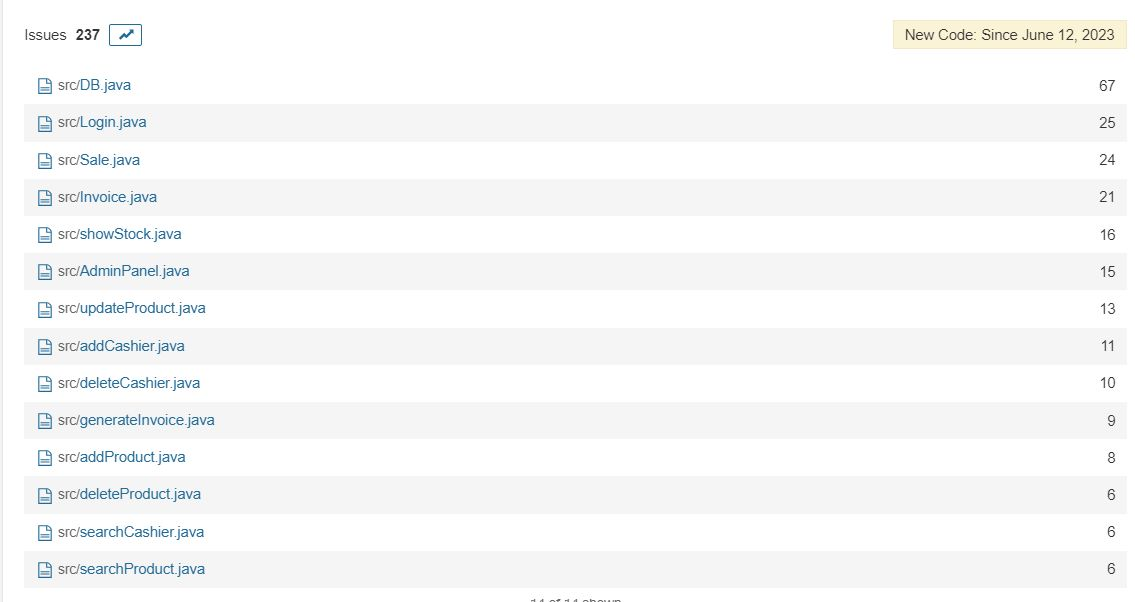
\includegraphics[width=1.0\linewidth]{Images/Before_Refactoring.jpeg}\
    \caption{Before Refactoring - Total Findings (Billing System)}
    \label{fig:enter-label}
    
\end{figure}
\pagebreak

\begin{figure}
    \centering
    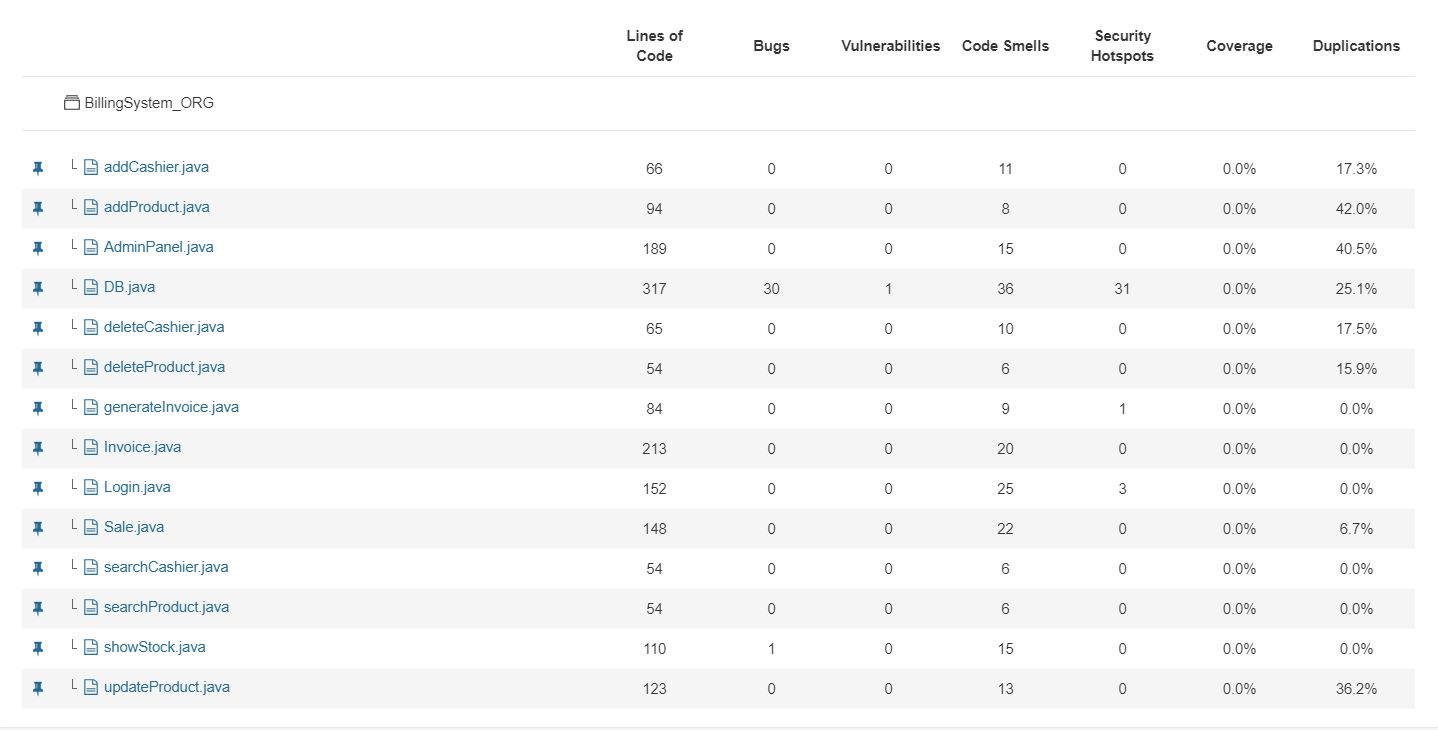
\includegraphics[width=1.0\linewidth]{Images/Quality_metrics_before.jpeg}\
    \caption{Before Refactoring - Quality Metrics (Billing System)}
    \label{fig:enter-label}
\end{figure}

\textbf{After Refactoring}

\begin{figure}[h!]
    \centering
    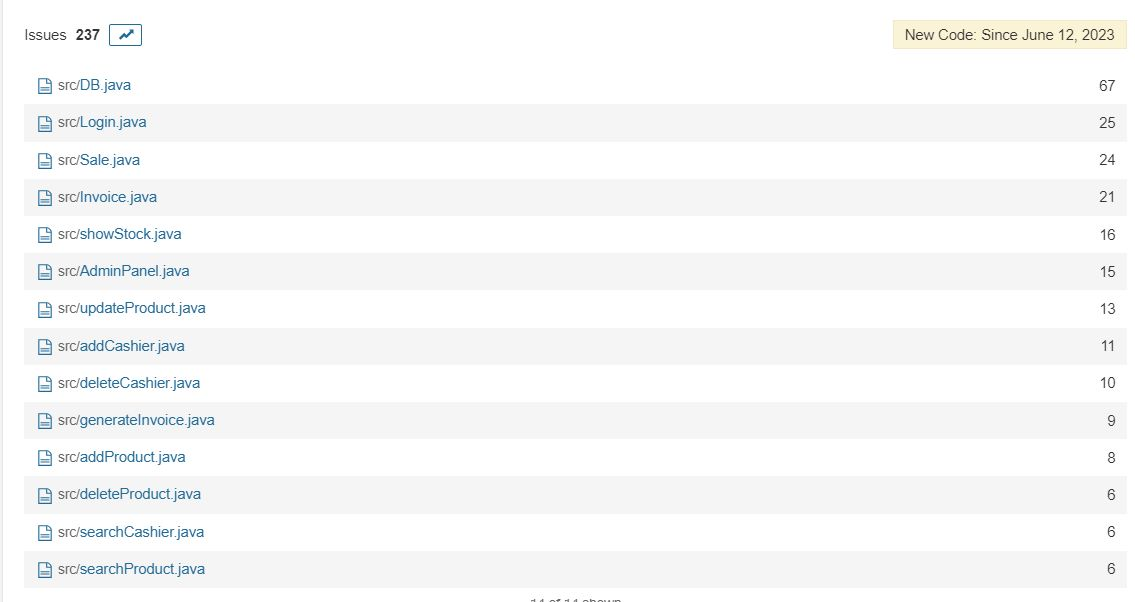
\includegraphics[width=1.0\linewidth]{Images/Before_Refactoring.jpeg}\
    \caption{After Refactoring - Total Findings (Billing System)}
    \label{fig:enter-label}
\end{figure}

\begin{figure}
    \centering
    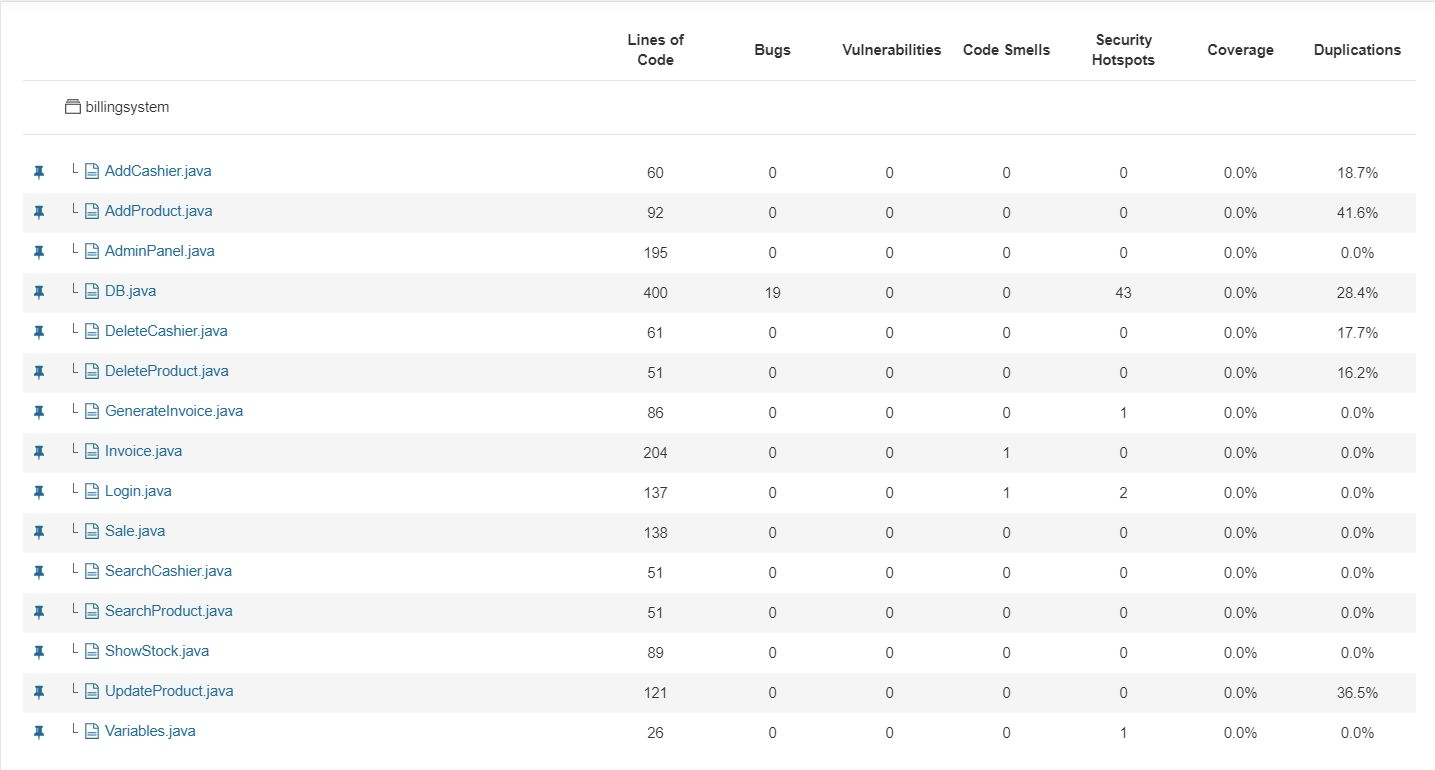
\includegraphics[width=1.0\linewidth]{Images/Quality_metrics_after.jpeg}\
    \caption{After Refactoring - Quality Metrics (Billing System)}
    \label{fig:enter-label}
\end{figure}

}

\pagebreak

\addcontentsline{toc}{section}{7. Refactoring Report}
\section*{7. Refactoring Report}

\normalsize{
In this comprehensive analysis, we present a detailed comparison between the state of the code before and after the refactoring process, taking into account various aspects such as technical debt and maintainability. By meticulously examining the codebase in both its pre-refactoring and post-refactoring states, we aim to shed light on the significant improvements achieved and the measures taken to address technical debt and enhance the overall maintainability of the software.\\

The decision to retain these 19 undesirables out of the initial 237 was taken with careful consideration, as altering them could potentially lead to changes in the system's core functionality as these 19 issues are false positive. Therefore, the focus was on prioritizing the issues based on their impact and criticality, ensuring that the essential functionalities remained intact while simultaneously improving the overall quality and performance of the system.\\

\begin{figure}[h!]
    \centering
    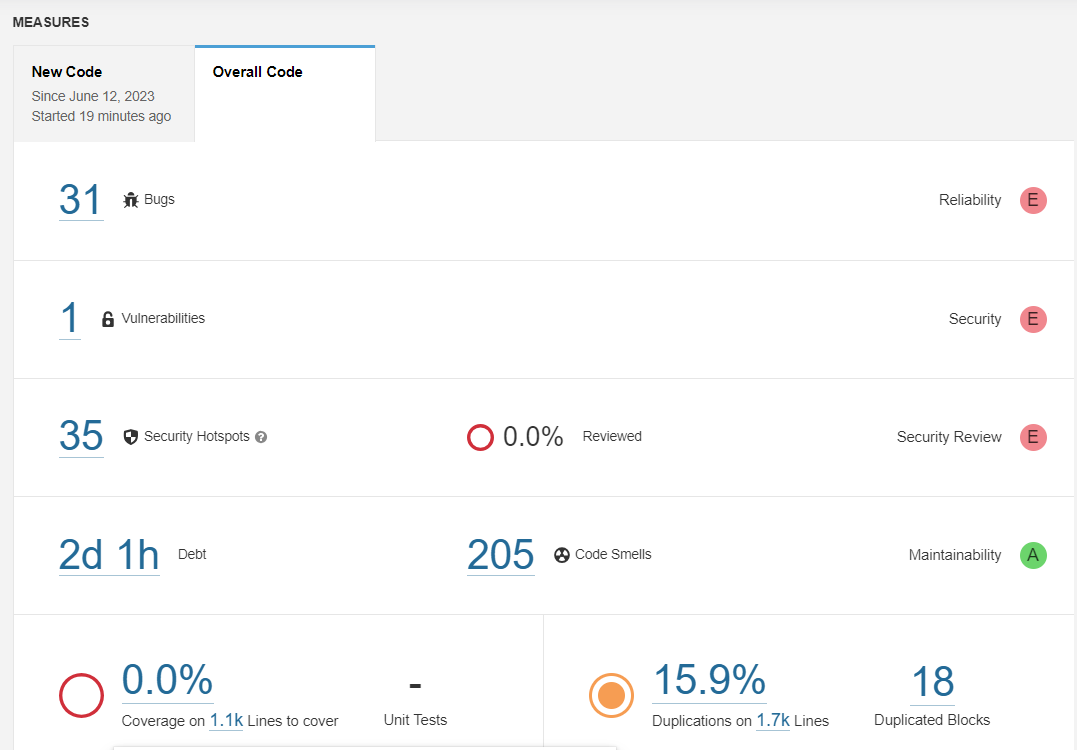
\includegraphics[width=0.9\linewidth]{Images/sonar_report.png}\
    \caption{SonarQube Report - Before Refactoring}
    \label{fig:enter-label}
\end{figure}

\begin{figure}[h!]
    \centering
    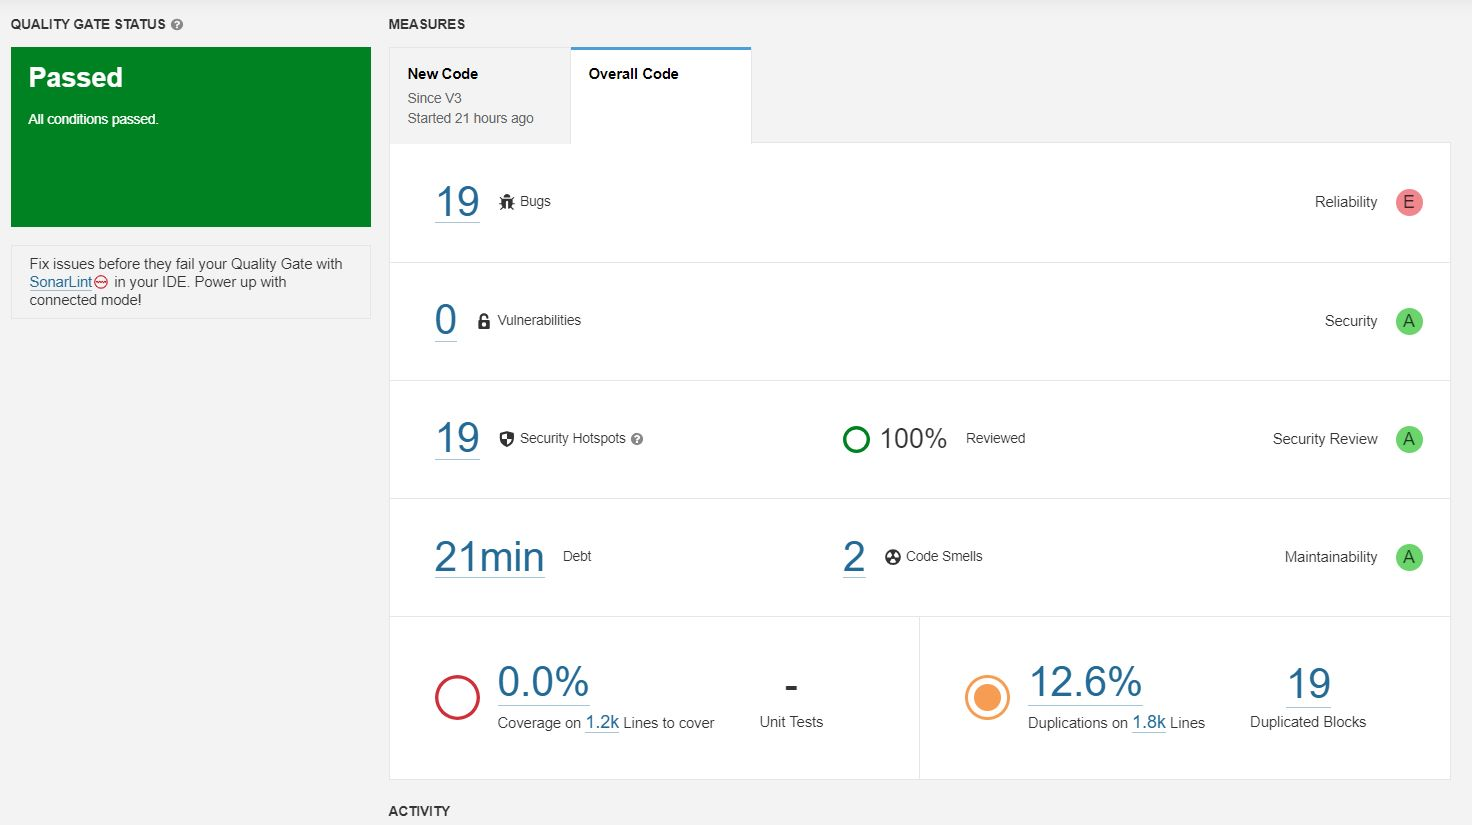
\includegraphics[width=0.9\linewidth]{Images/sonar_report_after.jpeg}\
    \caption{SonarQube Report - After Refactoring}
    \label{fig:enter-label}
\end{figure}


\begin{figure}[!tbp]
  \centering
  \subfloat[Before Refactoring]{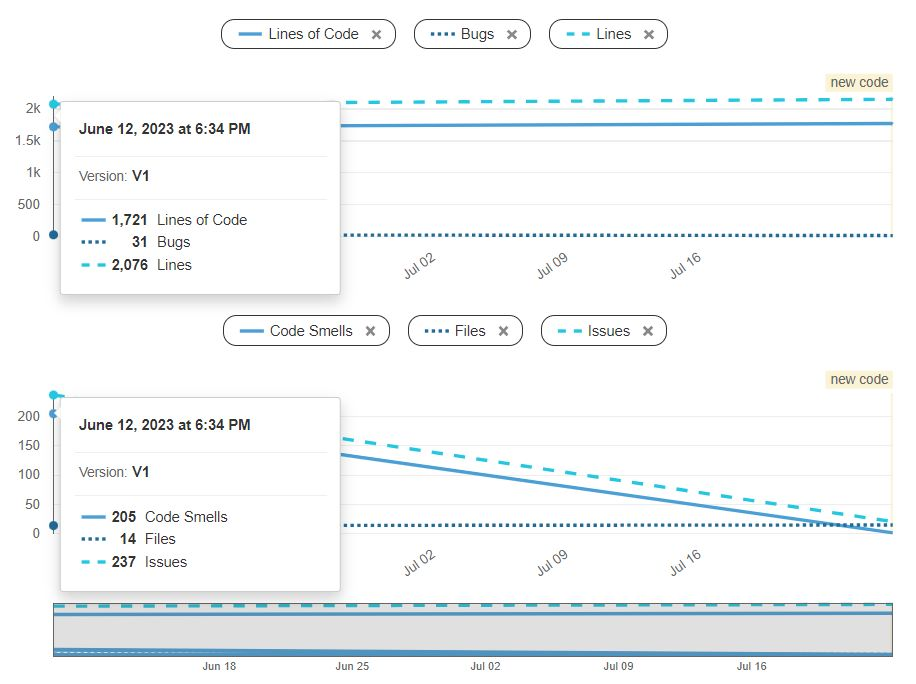
\includegraphics[width=0.5\textwidth]{Images/custom_metrics_before.jpeg}\label{fig:f1}}
  \hfill
  \subfloat[After Refactoring]{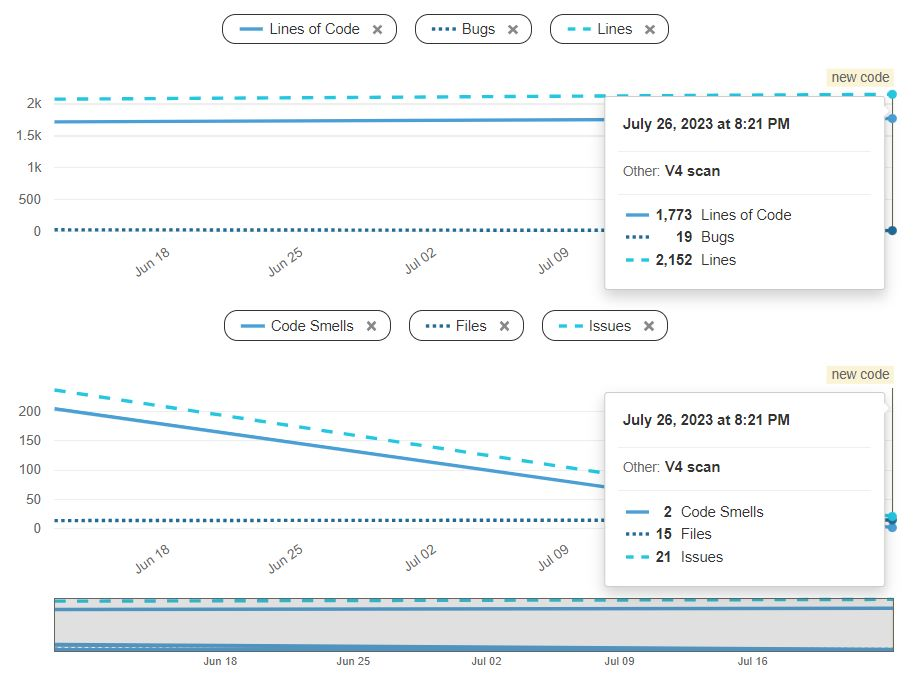
\includegraphics[width=0.5\textwidth]{Images/custom_metrics_after.jpeg}\label{fig:f2}}
  \caption{Comparison of Custom Metrics}
\end{figure}


\begin{figure}[!tbp]
  \centering
  \subfloat[Before Refactoring]{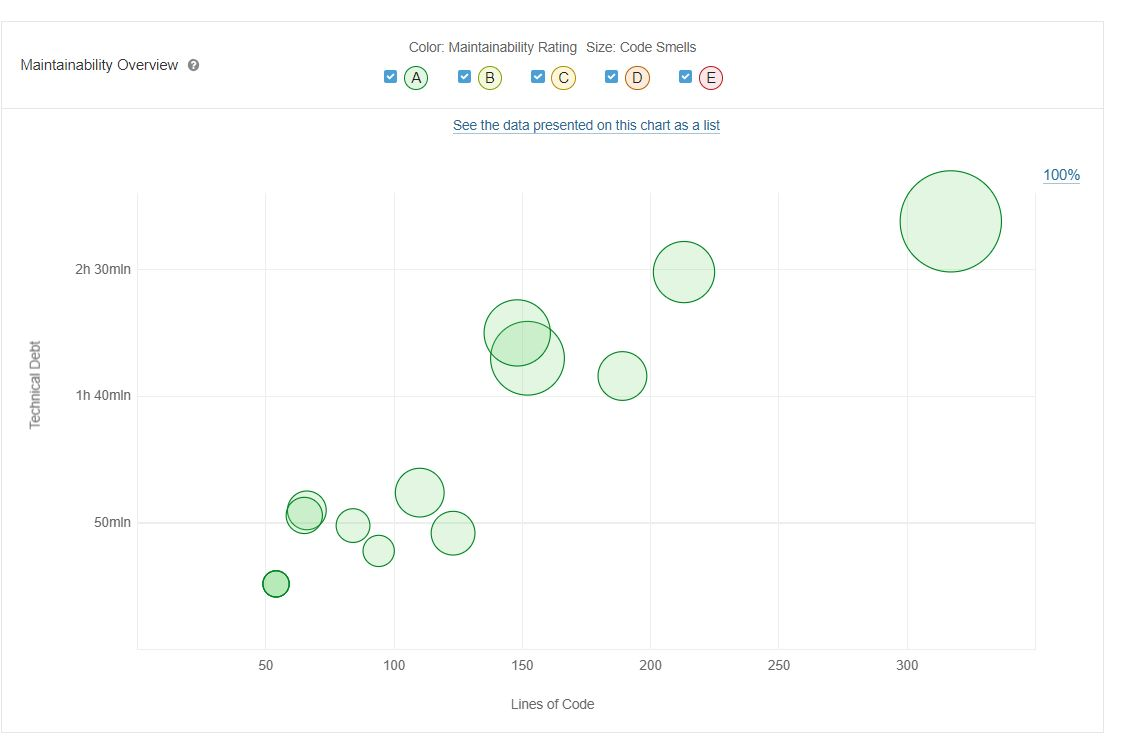
\includegraphics[width=0.5\textwidth]{Images/maintaininbility_before.jpeg}\label{fig:f1}}
  \hfill
  \subfloat[After Refactoring]{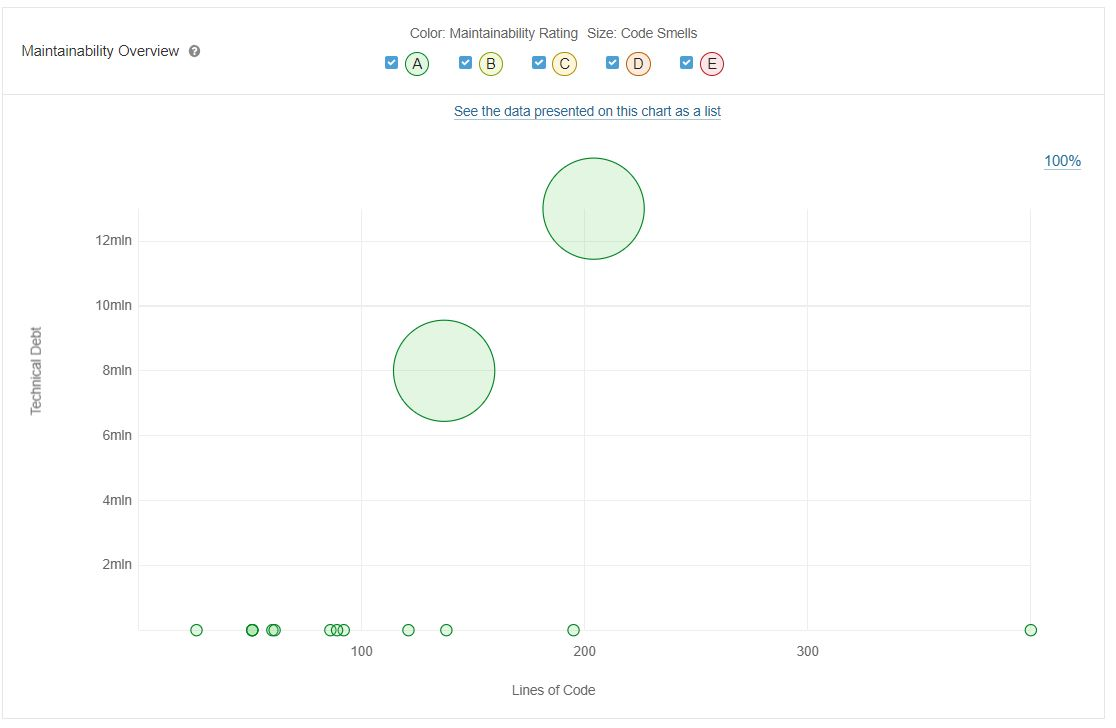
\includegraphics[width=0.5\textwidth]{Images/maintainibility_after.jpeg}\label{fig:f2}}
  \caption{Comparison of Maintainability}
\end{figure}

\begin{figure}[!tbp]
  \centering
  \subfloat[Before Refactoring]{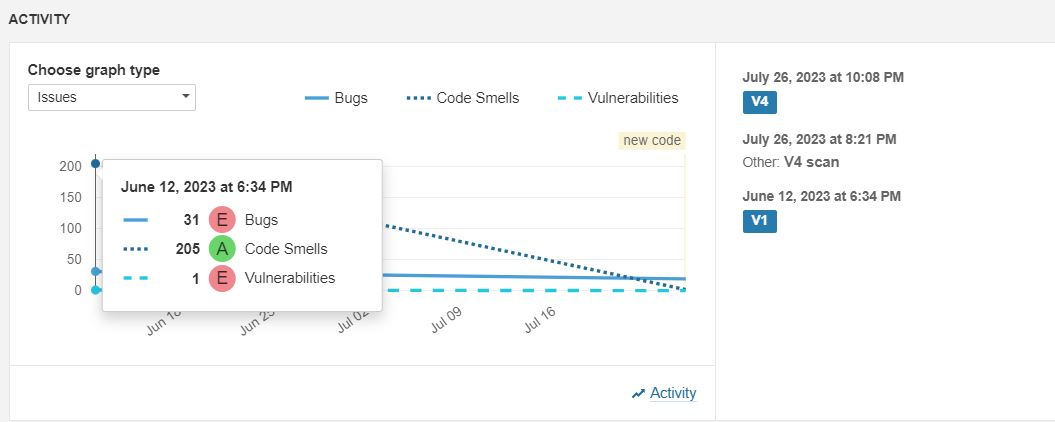
\includegraphics[width=0.5\textwidth]{Images/activity_graph_before.jpeg}\label{fig:f1}}
  \hfill
  \subfloat[After Refactoring]{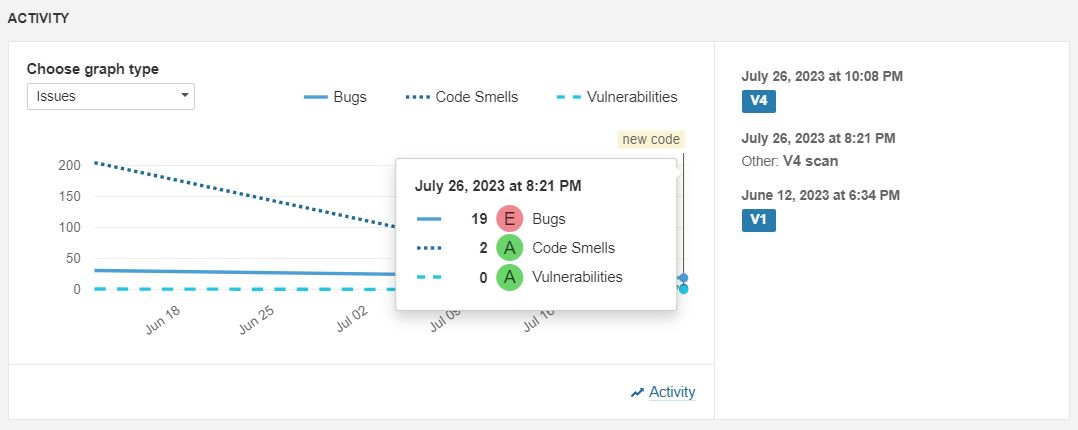
\includegraphics[width=0.5\textwidth]{Images/activity_graph_after.jpeg}\label{fig:f2}}
  \caption{Comparison of Activity Graphs}
\end{figure}

\begin{figure}[!tbp]
  \centering
  \subfloat[Before Refactoring]{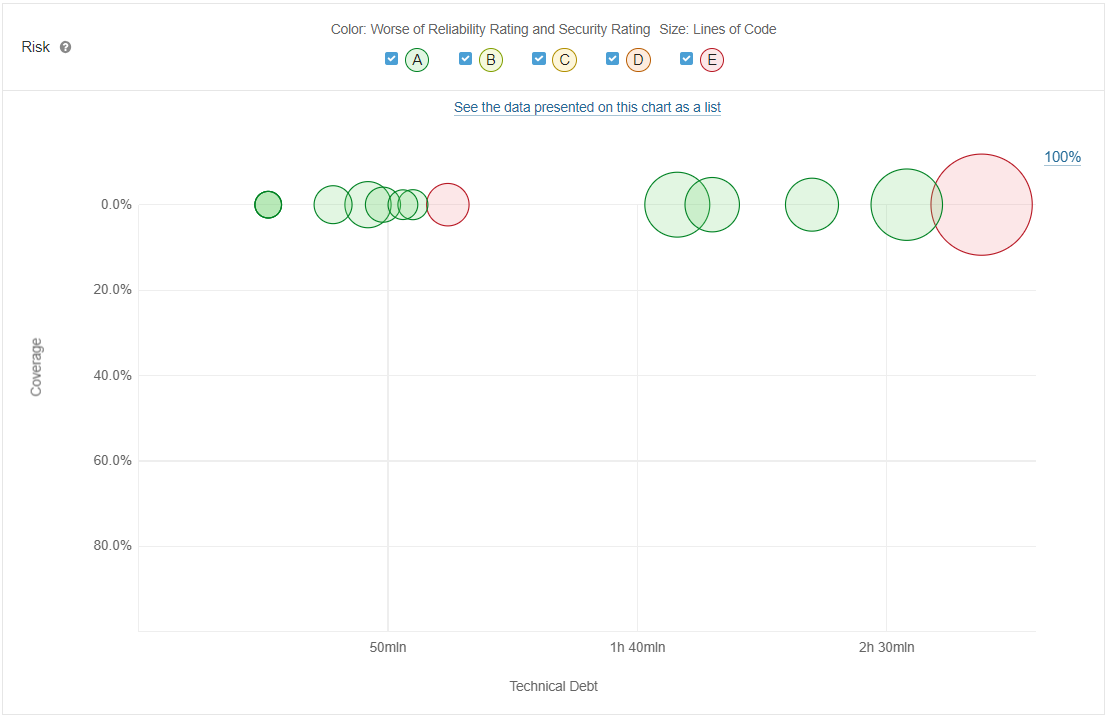
\includegraphics[width=0.5\textwidth]{Images/Debt_per_class.png}\label{fig:f1}}
  \hfill
  \subfloat[After Refactoring]{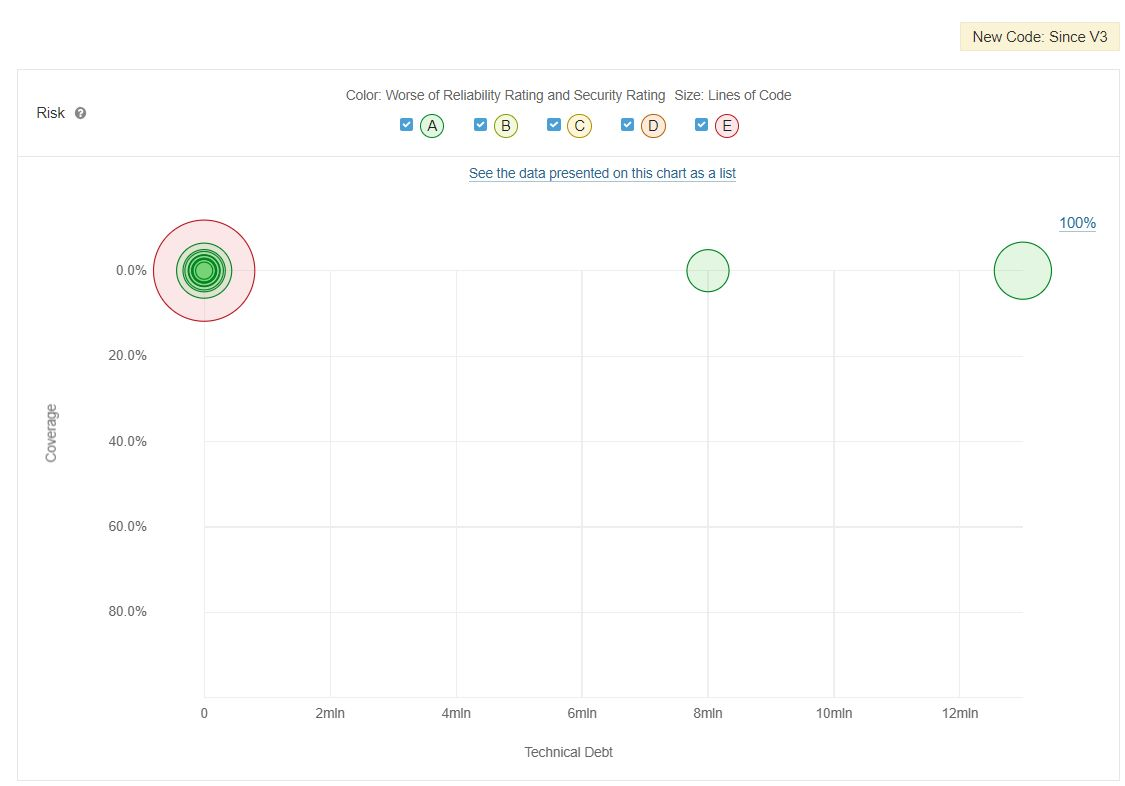
\includegraphics[width=0.5\textwidth]{Images/after_overview.jpeg}\label{fig:f2}}
  \caption{Comparison of Project Overview}
\end{figure}

}

\pagebreak

\addcontentsline{toc}{section}{8. Tools Used to Refactor the Candidate R}
\section*{8. Tools Used to Refactor the Candidate R}
\normalsize{

Below are the important tools we used to refactor Candidate R:\\
\begin{itemize}
    \item \textbf{Eclipse IDE}: The Eclipse IDE (Integrated Development Environment) is a popular software development tool that provides a rich set of features for coding, debugging, and testing applications. It is the second-most-popular IDE for Java development. It provides a powerful code editor with intelligent features like code completion, syntax highlighting, and code refactoring, which help increase productivity and maintain code quality. We used this for our code refactoring and its debugger helped us to improve the code quality in many ways.

    \item \textbf{Overleaf}: Overleaf is an online platform for collaborative writing and editing of documents, particularly focused on scientific and technical papers. It provides a user-friendly interface where writers can easily create and format their documents using LaTeX, a typesetting system commonly used for technical and scientific publications. We used overleaf collaboration feature so that we can work on the project document simultaneously and see each others edit in real time. 

    \item \textbf{GIT}: GIT, short for "Global Information Tracker," is a version control system that is used to track changes in files and directories. It allows multiple users to collaborate on a project by providing a way to manage and merge changes made by different individuals. We used GIT to organize our work and also reduce conflict during development. It also helped us to track changes made by different team members and provide facilities during merging code.

    \item \textbf{SonarQube}: SonarQube is an open-source platform used for continuous code quality inspection. We used this tool to detect issues related to code duplication, coding standards, security vulnerabilities, and bugs, among others. It also provides us with a range of metrics, including code coverage, complexity, and technical debt, which helps in tracking the progress of code quality improvement efforts.

    \item \textbf{Teamscale}: Teamscale is a software quality management platform that helps teams ensure the reliability and maintainability of their software projects. We analyzed code repositories using this and it  provided detailed insights into various code quality metrics such as code complexity, duplications, and coding standards violations. This helped us to identify areas that need improvement and to take appropriate actions to resolve potential issues.

   \item \textbf{VS Code}: VS Code, short for Visual Studio Code,is lightweight, efficient, and highly customizable code editor developed by Microsoft. It has very user-friendly interface and versatile features along with rich ecosystem of extensions. We used VS code for pair programming, debugging and code-refactoring.
    
\end{itemize}


\addcontentsline{toc}{section}{9. Source Code of Candidate System R}
\section*{9. Source Code of Candidate System R}

\normalsize{
In this particular segment, we have included the Source Code of the Candidate System R both prior to and following the completion of the Refactoring process.\\

\href{https://github.com/mdhruvi/SOEN-6431-Deja-Vu/tree/main/Selected%20System/Billing-System-master}{Source Code of Candidate R (Billing System) Before Refactoring}\\

\href{https://github.com/mdhruvi/SOEN-6431-Deja-Vu/tree/main/R%20after%20ReEngineering}{Source Code of Candidate R  (Billing System) After Refactoring}\\

}

\addcontentsline{toc}{section}{10. References}
\section*{10. References}
\href{https://iso25000.com/index.php/en/iso-25000-standards/iso-25010}{1. ISO/IEC 25010 Standard [Online].\\
 \href{https://ecomputernotes.com/software-engineering/coding-documentation}{2. Coding Documentation in Software Engineering [Online]. }\\
 \href{https://www.parasoft.com/blog/how-to-write-test-cases-for-software-examples-tutorial/}{3. William McMullin, How to Write Test Cases for Software, May 27, 2021. [Online].}.\\

\href{https://iso25000.com/index.php/en/iso-25000-standards/iso-25010}{1. ISO/IEC 25010 Standard  [Online].}\\
 \href{https://ece.uwaterloo.ca/~snaik/MYBOOK2/Ch4-Reengineering.ppt}{2. Software Reengineering Strategies [Online]. }\\
 \href{https://docs.teamscale.com/getting-started/visual-studio/}{3. Teamscale Integration for Visual Studio [Online]}.\\
 \href{https://adamtheautomator.com/vscode-live-share/}{4.  VSCode Live Share : A Great Way to Collaborate with Your Team [Online].}\\
 \href{https://docs.sonarsource.com/sonarqube/latest/?gads_campaign=SQ-Hroi-PMax&gads_ad_group=Global&gads_keyword=&gclid=CjwKCAjwq4imBhBQEiwA9Nx1BmT0DFJxLxrGR4HkMScw3mZ8HuqixcLNKv2gMpyEL0_cPtFbNXdzchoCzJYQAvD_BwE}{5. SonarQube 10.1 Documentation [Online].}\\
 \href{https://docs.teamscale.com/}{6. Teamscale Documentation [Online].}\\
 \href{https://www.ijera.com/papers/Vol6_issue9/Part-5/P0609058487.pdf}{7. 
Satya Sobhan Panigrahi,  Pappu Sharada,   Dr,Sujit Panda (2016). Software Engineering: Re-Engineering Metrics. International Journal of Engineering Research and Application,  Vol. 6, Issue 9, pp.84-87.}\\
 \href{https://git-scm.com/doc}{8. GIT Documentation [Online]}
\end{document}
